\documentclass[12pt]{article}
\usepackage{graphics,graphicx}
%\usepackage[dvips]{graphics,graphicx}
\DeclareGraphicsExtensions{.ps,.jpg,.eps,.pdf,.png}
\usepackage{amsmath}
\usepackage{url}
%\usepackage{secdot}
%\usepackage{natbib}
\usepackage{verbatim, moreverb}
\bibliographystyle{plain}

%Figure path

\newcommand{\figurepath}{./figures}
\newcommand{\figfiletype}{pdf}

% Define the hangref environment used for the References list:
\newenvironment{hangref}
  {\begin{list}{}{\setlength{\itemsep}{4pt}
  \setlength{\parsep}{0pt}\setlength{\leftmargin}{+\parindent}
  \setlength{\itemindent}{-\parindent}}}{\end{list}}

% Set the page margins to 1 inch all around:
\marginparwidth 0pt\marginparsep 0pt \topskip 0pt\headsep
0pt\headheight 0pt \oddsidemargin 0pt\evensidemargin 0pt
\textwidth 6.5in \topmargin 0pt\textheight 9.0in

\newtheorem{theorem}{Theorem}


%%%%Added by Leo%%%%
\newcounter{Fig}
\renewcommand{\theFig}{\arabic{Fig}}
\newcommand{\Fig}[2]{\refstepcounter{Fig} \label{#1}
                     {\small\bf Figure \theFig.} {\small\sl #2 \par}}

\setcounter{topnumber}{3}
\renewcommand{\topfraction}{.9}
\setcounter{bottomnumber}{3}
\renewcommand{\bottomfraction}{.9}
\setcounter{totalnumber}{4}
\renewcommand{\textfraction}{.1}
\setlength{\floatsep}{.25in} 
\setlength{\intextsep}{.25in}

\setlength{\fboxrule}{2\fboxrule} \setlength{\fboxsep}{3\fboxsep}

\newcommand{\Sa}{8pt}
\newcommand{\Sb}{0pt}

\renewcommand{\_}{{\char"5F}}
\renewcommand{\{}{{\char"7B}}
\renewcommand{\}}{{\char"7D}}
\renewcommand{\^}{{\char"0D}}

\let\accute= \'
\renewcommand{\'}{{\char"0D}}

\newcommand{\bfit}{\bfseries\itshape}

\newlength{\extopskip} \newlength{\exbottomskip}
\setlength{\exbottomskip}{1\baselineskip}
\addtolength{\exbottomskip}{-5.0pt}
\setlength{\extopskip}{1\exbottomskip}
\addtolength{\extopskip}{-1\parskip}

\newenvironment{Example}{\vspace{1\extopskip}\noindent\hspace*{2em}
                         \frenchspacing\small
                         \tt\begin{tabular}{@{}l@{}}}{
                         \end{tabular}\\[1\exbottomskip]}

\newcommand{\Titem}{\item[$\triangleright$]}
\newcommand{\Ditem}{\item[$\diamond$]}

\newenvironment{Itemize}{\begin{quote}\normalsize
   \baselineskip 20pt plus .3pt minus .1pt \begin{itemize}}
   {\end{itemize}\end{quote}}
   % Set path to folder containing figures
\newcommand{\FigureFolder}{figures}
 

\begin{document}

\title{Optimization Services 1.0 User's Manual }
\vskip 2in
\author{Robert Fourer, Jun Ma, Kipp Martin}
\maketitle

\begin{abstract}
This is the User's Manual for the Optimization Services (OS) project.  The objective of  (OS) is to provide a set of standards for representing optimization instances, results, solver options, and communication between clients and solvers in a distributed environment using Web Services. This COIN-OR project provides source code for libraries and executable programs that implement OS standards. See the Optimization Services (OS) Home Site for more information.
\end{abstract}


\newpage
\tableofcontents
\listoffigures
\listoftables
\hyphenation{com-plex-Type}










%\noindent\hrulefill
\newpage

\section{Introduction}

The objective of Optimization Services (OS) is to provide a set of standards for representing optimization instances, results, solver options, and communication between clients and solvers in a distributed environment using Web Services. This COIN-OR project provides source code for libraries and executable programs that implement OS standards. See the Optimization Services (OS) Home Site for more information.


\section{Download and Installation}

OS is released as open source code under the Common Public License (CPL). This project was created by Robert Fourer, Jun Ma, and Kipp Martin. The code has been written primarily by Jun Ma, Kipp Martin, Robert Fourer and Huanyuan Sheng, the first two are the COIN project leaders for OS. Below we describe different methods for obtaining the C++ source code and binaries. 

\subsection{Obtaining the Source Code Subversion Repository (SVN)}

The C++ source code can be obtained using Subversion.  Users with Unix operating systems will most likely have an svn client. For Windows users wishing to obtain and SVN client we recommend ***kipp fillin 

The OS project page with a Wiki is available at \url{projects.coin-or.org\OS}. Execute the following steps to get the source code using SVN.

\noindent {\bf Step 1:}  Connect to a directory where you want the OS project to go.  The following command will download the project into the directory COIN-OS

\begin{verbatim}
svn co https://projects.coin-or.org/svn/OS/stable/1.0 COIN-OS
\end{verbatim}

\noindent {\bf Step 2:}  Connect to the distribution root directory.

\begin{verbatim}
cd COIN-OS
\end{verbatim}


\noindent {\bf Step 3:} Run the configure script that will generate the makefiles. 

\begin{verbatim}
./configure
\end{verbatim}

\noindent {\bf Step 4:}  Run the make files.

\begin{verbatim}
make
\end{verbatim}

\noindent {\bf Step 5:} Run the unitTest.

\begin{verbatim}
make test
\end{verbatim}

Depending upon which third party software you have installed, the result of running the unitTest should look something like:


{\small
\begin{verbatim}
HERE ARE THE UNIT TEST RESULTS:

Solved problem avion2.osil with Ipopt
Solved problem HS071.osil with Ipopt
Solved problem rosenbrockmod.osil with Ipopt
Solved problem parincQuadratic.osil with Ipopt
Solved problem parincLinear.osil with Ipopt
Solved problem callBack.osil with Ipopt
Solved problem callBackRowMajor.osil with Ipopt
Solved problem parincLinear.osil with Clp
Solved problem p0033.osil with Cbc
Solved problem rosenbrockmod.osil with Knitro
Solved problem callBackTest.osil with Knitro
Solved problem parincQuadratic.osil with Knitro
Solved problem parincQuadratic.osil with Knitro
Solved problem p0033.osil with SYMPHONY
Solved problem parincLinear.osil with DyLP
Solved problem lindoapiaddins.osil with Lindo
Solved problem rosenbrockmod.osil with Lindo
Solved problem parincQuadratic.osil with Lindo
Solved problem wayneQuadratic.osil with Lindo
Test the MPS -> OSiL converter on parinc.mps usig Cbc
Test the AMPL nl -> OSiL converter on hs71.nl using LINDO
Test a problem written in b64 and then converted to OSInstance
Successful test of OSiL parser on problem parincLinear.osil
Successful test of OSrL parser on problem parincLinear.osrl
Successful test of prefix and postfix conversion routines on problem rosenbrockmod.osil
Successful test of all of the nonlinear operators on file testOperators.osil
Successful test of AD gradient and Hessian calculations on problem CppADTestLag.osil


CONGRATULATIONS! YOU PASSED THE UNIT TEST
\end{verbatim}
}

If you do not see
\begin{verbatim}
CONGRATULATIONS! YOU PASSED THE UNIT TEST
\end{verbatim}
then you have not passed the unitTest and hopefully some semi-inteligble error message was given. CONGRATULATIONS! YOUPASSEDD THE UNIT TEST


\noindent {\bf Step 6:}  Install the libraries.

\begin{verbatim}
make install
\end{verbatim}

This will install all of the libraries in the {\tt lib} directory under the distribution root. 


The above steps are fully tested on Mac/Unix, Linux, and on Windows using either MINGW/MSYS or CYGWIN. Popular compilers like gcc/g++ or windows native compiler cl.exe can all be used.

 Note if you download the OS package, you get these additional COIN-OR projects.
\begin{itemize}
\item Cbc \url{projects.coin-or.org\Cbc}
\item Clp  \url{projects.coin-or.org\Clp}
\item CppAD \url{projects.coin-or.org\CppAD}
\item Dylp \url{projects.coin-or.org\Dylp}
\item Osi \url{projects.coin-or.org\Osi}
\item SYMPHONY \url{projects.coin-or.org\SYMPHONY}
\end{itemize}


\subsection{Obtaining the Source Code From a Tarball}

\subsection{Obtaining a Visual Studio Project}

\subsection{Obtaining the Binaries}


\subsection{Platforms}


 \begin{tabular}{l|c|c|c|c|c|c|}
 &Mac&Linux&Cyg-gcc&Msys-cl&Msys-gcc&MSVS \\ \hline
AMPL-Client &x&x&&x&& \\ \hline
Cbc &x&x&x&x&& \\ \hline
Clp &x&x&x&x&& \\ \hline
Cplex &x&x&&&& \\ \hline
DyLP &x&x&x&x&& \\ \hline
Ipopt &x&x&&&& \\ \hline
Knitro &x&&&&& \\ \hline
Lindo &x&x&&x&& \\ \hline
SYMPHONY &x&x&x&x&& \\ \hline
 \end{tabular}
 
 \vskip 14pt
 
 
 {\large
 \noindent {\bf Platform Detail:}
 }
 
 \vskip 12pt
 
 \begin{tabular}{l|c|c|c|}
 & {\bf Operating System} & {\bf Compiler} & {\bf  Hardware} \\ \hline
 Mac &Mac OS X 10.4.9&gcc 4.0.1&Power PC \\   \hline
 Linux &Red Hat 3.4.6-8&gcc 3.4.6& Dell Intel 32 bit chip\\ \hline
 Cyg-gcc &Windows 2003 Server&gcc 3.4.4& Dell Intel 32 bit chip \\ \hline
 Msys-cl &Windows XP&Visual Studio 2003 &Dell Intel 32 bit chip \\ \hline
 Msys-gcc &&& \\ \hline
 MSVS &Windows XP&Visual Studio 2003 &Dell Intel 32 bit chip \\ \hline

 \end{tabular}
 

\section{The OS Project Components}

kipp -- don't forget to mention the schemas, data, xslt files, etc.

\subsection{Key Protocols}

Explain OSiL, OSrL, OSoL, and OSpL. Also, OSnL

\section{The OS Library Components}

\subsection{OSAgent}

The {\tt OSAgent}  part of the library is used to facilitate communication with remote solvers. It is not used if the solver is invoked locally (i.e. on the same machine). 

\subsection{OSCommonInterfaces}

\subsection{OSModelInterfaces}



\subsection{OSParsers}



\subsection{OSSolverInterfaces}


The {\tt OSSolverInterfaces} library is designed to facilitate linking the OS library with various solver APIs. We first describe how to take a problem instance in OSiL format and connect to a solver that has a COIN-OR OSI interface.  See the OSI project \url{www.projects.coin-or.org/Osi}.   We then describe hooking to the COIN-OR nonlinear code {\tt Ipopt.} See \url{www.projects.coin-or.org/Ipopt}.  Finally we describe hooking to two commercial solvers KNITRO and LINDO. 

The OS library has been tested with the following solvers using the Osi Interface.

\begin{itemize}
\item Cbc
\item Clp
\item Cplex
\item DyLP
\item Glpk
\item SYMPHONY
\end{itemize}

In the {\tt OSSolverInterfaces} library there is an abstract class {\tt DefaultSolver} that has the following key members:

\begin{verbatim}
std::string osil;
std::string osol;
std::string osrl;
OSInstance *osinstance;
OSResult  *osresult;
\end{verbatim}
and the pure virtual function
\begin{verbatim}
virtual void solve() = 0 ;	
\end{verbatim}
In order to use a solver through the COIN-OR {\tt Osi} interface it is necessary to an object in the {\tt CoinSolver} class which inherits from the {\tt DefaultSolver} class and implements the appropriate {\tt solve()} function.  We illustrate with the Clp solver.

\begin{verbatim}
DefaultSolver *solver  = NULL;
solver = new CoinSolver();
solver->m_sSolverName = "clp";
\end{verbatim}

Assume that the data file containing the problem has been read into the string {\tt osil} and the solver options are in the string {\tt osol}. Then the {\tt Clp} solver is invoked as follows.

\begin{verbatim}
solver->osil = osil;
solver->osol = osol;
solver->solve();
\end{verbatim}

Finally, get the solution in {\tt OSrL} format as follows

\begin{verbatim}
cout << solver->osrl << endl;
\end{verbatim}

Even though LINDO and KNITRO are commercial solvers and do not have a COIN-OR {\tt Osi} interface these solvers are used in exactly the same manner as a COIN-OR solver. For example, to invoke the LINDO solver we do the following.

\begin{verbatim}
solver = new LindoSolver();	
\end{verbatim}

Similarly for KNITRO and Ipopt. In the case of the KNITRO, the {\tt KnitroSolver} class inherits from both {\tt DefaultSolver} class and the KNITRO {\tt NlpProblemDef} class. See \url{Kipp -- put in Knitro manual link} for more information on the KNITRO solver C++ implementation and the {\tt NlpProblemDef} class. Similarly, for Ipopt the {\tt IpoptSolver} class inherits from both the  {\tt DefaultSolver} class and the Ipopt {\tt TNLP} class.  See \url{Kipp -- put in Ipopt manual link} for more information on the Ipopt solver C++ implementation and the {\tt TNLP} calss.

In the examples above the problem instance was assumed to be read from a file into the string {\tt osil} and then into the class member {\tt solver->osil.} However, everything can be done entirely in memory. For example, it is possible to use the {\tt OSInstance} class to create an in-memory problem representation and give this representation directly to a solver class that inherits from {\tt DefaultSolver}. The class member to use is {\tt osinstance.} This is illustrated in the example given in Section \ref{subsection:exampleOSInstance}.


\subsection{OSUtils}

\section{OSInstance: A General Instance API}

\subsection{Get Methods}

\subsection{Set Methods}

\subsection{Calculate Methods}

\section{Hooking to An Algorithmic Differentiation Package}

\section{The OSSolverService}

The {\tt OSSolverService} is a command line executable designed to pass problem instances to solvers and get the result back to be displayed either to standard output or a specified browser.  The {\tt OSSovlerService} can be used to invoke a solver locally or on a remote server. It can work either synchronously or asynchronously. 

\subsection{OSSolverService Input Parameters}

At present, the {\tt OSSolverService} takes the following parameters. The order of the parameters is irrelevant.  Not all the parameters are required. However, two pieces of information {\it must} be contained in the input paramters.  First,  the problem instance location must be specified (either locally or on a remote machine). Second, the solver must be specified. 

\begin{itemize}

\item[] {\bf -osil xxx.osil}  this is the name of the file that contains the optimization instance in OSiL format. It is assumed that this file is available in a directory on the machine that is running {\tt OSSolverService}. If this option is not specified then the instance location must be specified in the OSoL solver options file.

\item[] {\bf -osol xxx.osol}  this is the name of the file that contains the solver options. It is assumed that this file is available in a directory on the machine that is running {\tt OSSolverService}. It is not necessary to specify this option.

\item[] {\bf -osrl xxx.osrl}  this is the name of the file that contains the solver solution. A valid file path must be given on the machine that is running {\tt OSSolverService}. It is not necessary to specify this option.

\item[] {\bf -serviceLocation}  is the URL of the solver service. This is not required, and if not specified it is assumed that the problem is solved locally. 

\item[] {\bf -serviceMethod  method}  this is  the solver service required. The options are {\tt solve}, {\tt send},{\tt kill},{\tt knock}, {\tt getJobID}, and {\tt retrieve}. The use of these options is illustrated in the examples below. This option is not required, and the default value is {\tt sovle.}

\item[] {\bf -mps  xxx.mps}  this is the name of the mps file if the problem instance is in mps format. It is assumed that this file is available in a directory on the machine that is running {\tt OSSolverService}. The default file format is OSiL so this option is not required.

\item[] {\bf -nl  xxx.nl}  this is the name of the AMPL nl file if the problem instance is in AMPL nl  format. It is assumed that this file is available in a directory on the machine that is running {\tt OSSolverService}. The default file format is OSiL so this option is not required.

\item[] {\bf -solver  solverName} this parameter is required if the problem is solved locally. Possible values for default OS installation are {tt clp} (COIN-OR Clp), {\tt cbc} (COIN-OR Cbc), {\tt dylp} (COIN-OR DyLP), and {\tt symphony} (COIN-OR SYMPHONY). Other solvers supported (if the necessary libraries are present) are {\tt cplex} (Cplex through COIN-OR Osi), {\tt glpk} (glpk through COIN-OR Osi), {\tt ipopt} (COIN-OR Ipopt),  {\tt knitro} (Knitro), and {\tt lindo} {\tt LINDO}.


\item[] {\bf -browser  browserName} this paramater is a path to the browser on the local machine. If this optional parameter is specified then the solver result in OSrL format is transformed using XSLT into HTML and displayed in the browser. 

\item[] {\bf -config pathToConfigureFile} this parameter specifies a path on the local machine to a text file containing values for the input parameters. This is convenient for the user not wishing to constantly retype parameter values.



\end{itemize}


{\bf Some Rules:}

\begin{itemize}
\item[1.]  When using the {\tt send()} or  {\tt solve()} methods a problem instance file location {\it must} be specified either at  the command line, in the configuration file, or in the {\tt <instanceLocation>} element in the OSoL options file file.

\item[2.]  The {\tt serviceMethod} option must be specified at the command line or in a configuration file.  The service method cannot be specified in the OSoL options file. 

\item [3.]  If the {\tt solver} option is not specified, the COIN-OR solver {\tt Cbc} is the default solver used. In this case an error is thrown if the problem instance has quadratic or other nonlinear terms. 

\item[4.]  If the options ={\tt send}, {\tt kill}, {\tt knock},  {\tt getJobID},  or {\tt retrieve} are specified, a  {\tt serviceLocation} must be specified. 

\item[5.]  The default {\tt serviceMethod} used is {\tt solve} if one is not specified.

\item[6.] When calling a remote server, the solver option must be specified in the {\tt OSoL} file.
\end{itemize}



The input parameters to the {\tt OSSolverService} may be given entirely in the command line or in a configuration file.  We first illustrate giving all the  parameters in the command line. The following command will invoke the {\tt Clp} solver on the local machine to solve the problem instance {\tt parincLinear.osil}.

\begin{verbatim}
OSSolverService -solver clp -osil ../data/parincLinear.osil 
\end{verbatim}

Alternatively, these parameters can be put into a configuration file. Assume that the configuration file of interest is {\tt testlocalclp.config}. It would contain the two lines of information
\begin{verbatim}
-osil ../data/parincLinear.osil
-solver clp
\end{verbatim}
Then the command line is
\begin{verbatim}
OSSolverService -config ../data/testlocalclp.config
\end{verbatim}


Parameters specified in the configure file are overridden by parameters specified at the command line. This is convenient if a user has a base configure file and wishes to override only a few options. For example,
\begin{verbatim}
OSSolverService -config ../data/testlocalclp.config -solver lindo
\end{verbatim}
or
\begin{verbatim}
OSSolverService -solver lindo -config ../data/testlocalclp.config 
\end{verbatim}
will result in the LINDO solver being used even though Clp is specified in the {\tt testlocalclp} configure file.

\subsection{Solving Problems Locally}

Generally, when solving a problem locally the user will use the {\tt solve} service method. The {\tt solve} method is invoked synchronously and waits for the solver to return the result. The {\tt sovle} method has two arguments. The first argument is the OSoL file path and the second argument is the OSiL file path. The OSoL file path may be empty.  Here is an illustration of using a configure file,  {\tt testlocal.config}, to invoke {\tt Ipopt} locally.

\begin{verbatim}
-osil ../data/parincQuadratic.osil
-solver ipopt
-serviceMethod solve
-browser /Applications/Firefox.app/Contents/MacOS/firefox
-osrl /Users/kmartin/temp/test.osrl
\end{verbatim}

The first line of {\tt testlocal.config} gives the local location of the OSiL file, {\tt parincQuadratic.osil}, that contains the problem instance. The second parameter, {\tt -solver ipopt},  is the solver to be invoked. The third parameter {\tt -serviceMethod solve} is not really needed, but included only for purpose of illustration. The default  solver service is {\tt solve.}  The fourth parameter is the location of the browser on the local machine. It will read the OSrL file on the local machine using the path specified by the value of the {\tt osrl} parameter, in this case {\tt /Users/kmartin/temp/test.osrl.}

In the configuration file {\tt testlocalosol.config} we illustrate specifying the instance location in an OSoL file.

\begin{verbatim}
-osol ../data/demo.osol
-solver clp
\end{verbatim}

The file {\tt demo.osol} is

\begin{verbatim}
<?xml version="1.0" encoding="UTF-8"?>
<osol xmlns="os.optimizationservices.org"
xmlns:xs="http://www.w3.org/2001/XMLSchema"
xmlns:xsi="http://www.w3.org/2001/XMLSchema-instance"
xsi:schemaLocation="os.optimizationservices.org 
http://www.optimizationservices.org/schemas/OSoL.xsd">
  <general>         
       <instanceLocation locationType="local">
       ../data/parincLinear.osil
       </instanceLocation>
  </general>
</osol>
\end{verbatim}

\subsection{Solving Problems Remotely with Web Services}

We now illustrate using the {\tt OSSolverService} executable to call a remote solver service.  
By remote solver service we mean a solver service that is called using Web services.  
Both the  {\tt OSSolverService} and the Web service could be on the same physical machine.

In the following sections we illustrate each of the six service methods.  All of these examples are based upon a solver service running on a remote server running Apache Tomcat. See \url{tomcat.apache.org}. The Web Service running on the server is a Java program based on Apache Axis. See \url{ws.apache.org/axis}. This is described in greater detail in Section \ref{section:tomcat}.  This Web Service is called {\tt OSSolverService.jws}. This Java program calls a C++ executable OSSolverService on the server. So there is an OSSolverService on the client that calls the Web Service {\tt  OSSolverService.jws} that in turn calls  the executable {\tt OSSovlerService} on the server.  See Figure \ref{figure:ossolverservice}.
 
\begin{figure}
\centering
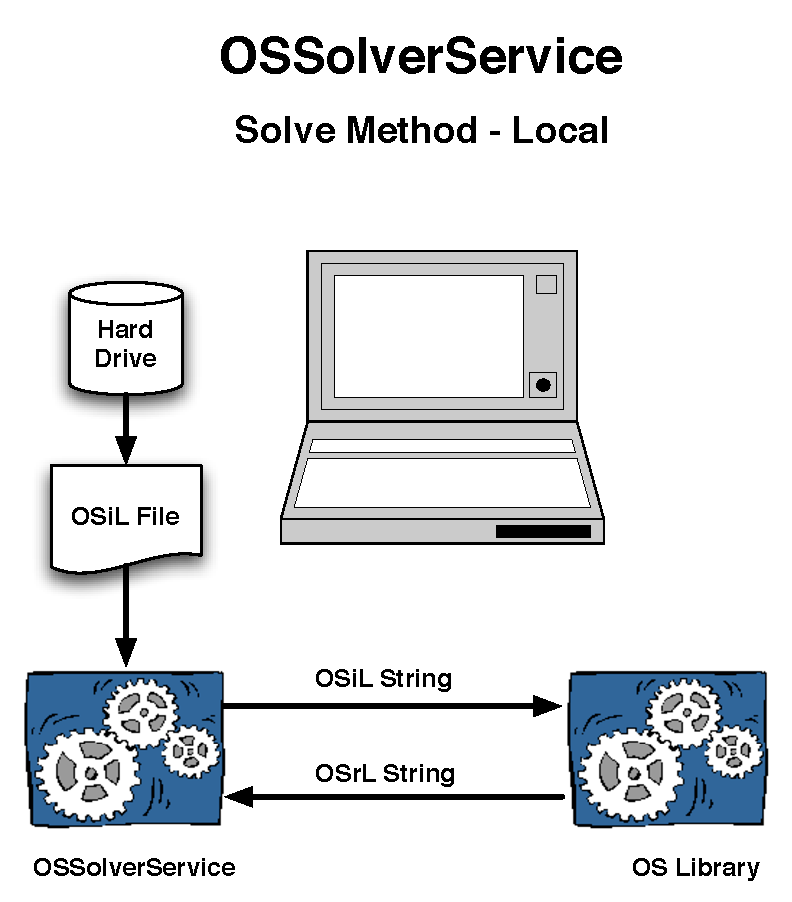
\includegraphics[scale=0.25]{\figurepath/OSSolverServiceLocal.pdf}
\caption{A remote call to {\tt solve}.} 
\label{figure:ossolverservice}
\end{figure}


\subsubsection{The  {\tt solve} Service Method}\label{section:solve}

First we illustrate a simple call to   {\tt OSSolverService.jws} and request a solution using the COIN-OR  {\tt Clp} solver.  The call on the client machine is

\begin{verbatim}
OSSolverService -config ../data/testremote.config
\end{verbatim}
where the {\tt testremote.config} file is
\begin{verbatim}
-osil ../data/parincLinear.osil
-serviceLocation http://128.135.130.17:8080/os/OSSolverService.jws
\end{verbatim}

No solver is specified so by default the  {\tt Cbc} solver will be used on the server.  

Now use an OSoL options file
\begin{verbatim}
OSSolverService -osol ../data/remoteSolve1.osol -osil ../data/parincLinear.osil
\end{verbatim}
where {\tt remoteSolve1.osol} is
\begin{verbatim}
<?xml version="1.0" encoding="UTF-8"?>
<osol xmlns="os.optimizationservices.org">
    <general>
        <serviceURI>http://128.135.130.17:8080/os/OSSolverService.jws</serviceURI>
    </general>
    <optimization>
    	<other name="os_solver">clp</other>
    </optimization>
</osol>
\end{verbatim}
In this case we specify a sover to use, name {\tt Clp}.

Next we illustrate a call to the remote SolverService and specify an OSiL instance that is on the remote machine.
\begin{verbatim}
OSSolverService -osol ../data/remoteSolve2.osol
\end{verbatim}
where the {\tt remoteSolve2.osol} file is
\begin{verbatimtab}[4]
<?xml version="1.0" encoding="UTF-8"?>
<osol xmlns="os.optimizationservices.org">
    <general>
        <serviceURI>http://128.135.130.17:8080/os/OSSolverService.jws</serviceURI>
         <instanceLocation locationType="local">
	 /home/kmartin/files/code/OSRepository/linear/continuous/pilot.osil
	 </instanceLocation>
    </general>
    <optimization>
    	<other name="os_solver">clp</other>
    </optimization>
</osol>
\end{verbatimtab}
if we were to change to the {\tt locationType} attribute in the {\tt <instanceLocation>} element to {\tt http} then we could specify the intance location to on yet another machine. This is illustrate below  for {\tt remoteSovle3.osol}.
\begin{verbatimtab}[4]
<?xml version="1.0" encoding="UTF-8"?>
<osol xmlns="os.optimizationservices.org">
    <general>
        <serviceURI>http://128.135.130.17:8080/os/OSSolverService.jws</serviceURI>
         <instanceLocation locationType="http">
	 http://gsbkip.chicagogsb.edu/testproblems/parincLinear.osil
	 </instanceLocation>
    </general>
    <optimization>
    	<other name="os_solver">clp</other>
    </optimization>
</osol>
\end{verbatimtab}

kipp illustrate the above with a figure






Illustrate when data is uploaded locally or when data is uploaded from another server. 

\subsubsection{The  {\tt send} Service Method}\label{section:send}

When the {\tt solve} service method is used, the {\tt OSSolverService} does not finish execution until the solution is returned from the remote solver service. The {\tt solve} method communicates synchronously with the remote solver service. This may not be desirable for large problems when the user does not want to wait for a response. The {\tt send} service method should be used when asynchronous communication is desired. When the send method is used the instance is communicated to the remote service and the {\tt OSSolverService} terminates after submission. An example of this is
\begin{verbatim}
OSSolverService -config ../data/testremoteSend.config
\end{verbatim}
where the {\tt testremoteSend.config} file is
\begin{verbatim}
-solver ipopt
-nl ../data/hs71.nl
-serviceLocation http://128.135.130.17:8080/os/OSSolverService.jws
-serviceMethod send
\end{verbatim}
In this example the COIN-OR {\tt Ipopt} solver is specified. The input file {\tt hs71.nl} is in AMPL format. Before sending this to the remote solver service the {\tt OSSolverService} executable converts  the nl format into the OSiL XML format and packages this into the SOAP envelope used by Web Services. 

Since the {\tt send} method involves asynchronous communication the remote solver service must keep track of jobs. The send methd requires a {\tt JobID}. In the above example  no {\tt JobID} was specified. When no {\tt JobID} is specified the {\tt OSSolverService} method first invokes the {\tt getJobID} service method to get a {\tt JobID} and then puts this information into a created OSoL file and send the information to the server. More information on the {\tt getJobID} service method is provided in Section \ref{section:getjobid}.  The {\tt OSSolverService} prints the OSoL file to standard output before termination. This is illustrated below,
\begin{verbatimtab}[4]
<?xml version="1.0" encoding="UTF-8"?> 
<osol xmlns="os.optimizationservices.org">
	<general> 
		<jobID>
		gsbrkm4__127.0.0.1__2007-06-16T15.46.46.075-05.00149771253
		</jobID>
	</general>
</osol>
\end{verbatimtab}
The {\tt JobID} is one that is randomly generated by the server and passed back to the {\tt OSSolverService.} The user can also provide a {\tt JobID} in their OSoL file. For example, below is a user-provided OSoL file that could be specified in a configuration file or on the command line.
\begin{verbatimtab}[4]
<?xml version="1.0" encoding="UTF-8"?>
<osol xmlns="os.optimizationservices.org">
	<general>  
		<jobID>123456abcd</jobID>       
	</general>
</osol>
\end{verbatimtab}

In order to be of any use, it is necesary to get the result of the optimization. This is described in Section \ref{section:retrieve}. Before proceeding to this section, we describe two ways for knowing when the optimization is complete. One feature of the standard OS remote SolverService is the ability to send an email when the job is complete. Below is an example of the {\tt OSoL} that uses the email feature.
\begin{verbatimtab}[4]
<?xml version="1.0" encoding="UTF-8"?>
<osol xmlns="os.optimizationservices.org">
 	<general>  
 		<jobID>123456abcd</jobID>   
 		<contact transportType="smtp">
			kipp.martin@chicagogsb.edu
		</contact>     
	</general>
</osol>
\end{verbatimtab}

The remote Solver Service will send an email to the above address when the job is complete. A second option for knowing when a job is complete is to use the knock method. 



\subsubsection{The  {\tt retrieve} Service Method}\label{section:retrieve}

The {\tt retrieve} has a single string argument which is an OSoL instance. Here is an example of using the {\tt retrieve} method with {\tt OSSolverService}.
\begin{verbatim}
OSSolverService -config ../data/testremoteRetrieve.config
\end{verbatim}
The {\tt testremoteRetrieve.config} file is
\begin{verbatim}
-serviceLocation http://128.135.130.17:8080/os/OSSolverService.jws
-osol ../data/retrieve.osol
-serviceMethod retrieve
-osrl /home/kmartin/temp/test.osrl
\end{verbatim}
and the {\tt retrieve.osol} file is
\begin{verbatimtab}[4]
<?xml version="1.0" encoding="UTF-8"?>
<osol xmlns="os.optimizationservices.org">
 	<general>         
 		<jobID>123456abcd</jobID>  
	</general>
</osol>
\end{verbatimtab}
The OSoL file {\tt retrieve.osol} contains a tag {\tt <jobID>} that is communicated to the remote service. The remove service locates the result returns it as a string. The string that is returned is an OSrL instance. 

\subsubsection{The  {\tt getJobID} Service Method}\label{section:getjobid}

Before  submitting a job with the {\tt send} method a {\tt JobID} is required. The {\tt OSSolverService} can get a {\tt JobID} as follows
\begin{verbatim}
-serviceLocation http://128.135.130.17:8080/os/OSSolverService.jws
-serviceMethod getJobID
\end{verbatim}
Note that no OSoL input file is specified. In this case, the {\tt OSSolverService} sends an empty string. A string is returned with the {\tt JobID}. This {\tt JobID} is then put into a {\tt <jobID>} element in an OSoL string that would be used by the {\tt send} method.


\subsubsection{The  {\tt knock} Service Method}\label{section:knock}

The OSSolverService terminates after executing the {\tt send} method. Therefore, it is necessary to know when the job is completed on the remote server. One way is to include an email address in the  {\tt <contact>}  element with the attribute {\tt transportType}     set to {\tt smtp}.  This was illustrated in Section \ref{section:solve}.  A second way to check on the status of a job is to use the {\tt knock} service method.  For example, assume a user   wants to know if  the job with {\tt JobID 123456abcd}  is complete. A user would make the request
\begin{verbatim}
OSSolverService -config ../data/testRemoteKnock.config
\end{verbatim}
where the {\tt testRemoteKnock.config} file is
\begin{verbatim}
-serviceLocation http://128.135.130.17:8080/OS/OSSolverService.jws
-osplInput ../data/demo.ospl
-osol ../data/retrieve.osol
-serviceMethod knock
\end{verbatim}
the {\tt demo.ospl} file is
\begin{verbatim}
<?xml version="1.0" encoding="UTF-8"?>
<ospl xmlns="os.optimizationservices.org">
<processHeader>
<request action="getAll"/>
</processHeader>
<processData/>
</ospl>
\end{verbatim}
and the {\tt retrieve.osol} file is
\begin{verbatim}
<?xml version="1.0" encoding="UTF-8"?>
<osol xmlns="os.optimizationservices.org">
 	<general>         
 		<jobID>123456abcd</jobID>  
	</general>
</osol>
\end{verbatim}
The result of this request is a string in OSrL format.  Part of the return format is illustrated below.
\begin{verbatimtab}[4]
<jobs>
	<job jobID="123456abcd">
		<state>finished</state>
		<serviceURI>http://128.135.130.17:8080/ipopt/IPOPTSolverService.jws</serviceURI>
		<submitTime>2007-06-16T14:57:36.678-05:00</submitTime>
		<startTime>2007-06-16T14:57:36.678-05:00</startTime>
		<endTime>2007-06-16T14:57:39.404-05:00</endTime>
		<duration>2.726</duration>
 </job>
</jobs>
\end{verbatimtab}
Notice the {\tt <state>} element indicating that the job is finished.   

When making a {\tt knock} request,  the OSoL string can be empty. In this example, if the OSoL string had been empty the status of all jobs solved since the disk clean-up would get reported.  Also, there are values other than {\tt getAll} for the OSpL {\tt action} attribute in the {\tt <request>} tag.  For example, the {\tt action} can be set to a value of {\tt ping} if the user just wants to check if the remote solver service is up and running. 



\subsubsection{The  {\tt kill}   Service Method}

If the user submits a job that is taking too long or is a mistake it is possible to kill the job on the remote server using the {\tt kill} service method. For example to kill job {\tt 123456abcd} .  At the command line type
\begin{verbatim}
OSSolverService -config  ../data/kill.config
\end{verbatim}
where the configure file {\tt kill.config} is
\begin{verbatim}
-osol ../data/kill.osol
-serviceLocation http://128.135.130.17:8080/os/OSSolverService.jws
-serviceMethod kill
\end{verbatim}
and the {\tt kill.osol} file is
\begin{verbatimtab}[4]
<?xml version="1.0" encoding="UTF-8"?>
<osol xmlns="os.optimizationservices.org">
 	<general>         
 		<jobID>123456abcd</jobID>  
	</general>
</osol>
\end{verbatimtab}


\subsubsection{Summary}

Below is a summary of the inputs and outputs of the six service methods. See also Figures \ref{figure:async1} and \ref{figure:async2}.

\begin{itemize}
\item {\tt solve(osil, osol):}

\begin{itemize}

\item Inputs: a string with the instance in OSiL format and a string with the solver options in OSoL format

\item  Returns: a string with the solver solution in OSrL format

\item  Synchronous call, blocking request/response

\end{itemize}



\item {\tt send(osil, osol)}


\begin{itemize}

\item Inputs: a string with the instance in OSiL format and a string with the solver options in OSoL format

\item Returns:  a boolean, true if the problem was successfully submitted, false otherwise

\item Has the same signature as {\tt solve}

\item  Asynchronous (server side), non-blocking call

\item The {\tt osol} string should have a {\tt JobID} in the {\tt <jobID>} element
\end{itemize}

\item {\tt getJobID( osol)}

\begin{itemize}

\item Inputs: a string  with the solver options in OSoL format (in this case, the string may be empty because no options are required to get the JobID)

\item  Returns: a string which is the unique job id generated by the solver service

\item  Used to maintain session and state on a distributed system
\end{itemize}



\item {\tt knock(ospl, osol)}

\begin{itemize}

\item Inputs: a string in OSpL format and a string with the solver options in OSoL format

\item  Returns: process and job status information from the remote server in OSpL format

\end{itemize}

\item {\tt retrieve( osol)}


\begin{itemize}

\item Inputs: a string with the solver options  in OSoL format  

\item Returns: a string with the solver solution in OSrL format

\item The {\tt osol} string should have a {\tt JobID} in the {\tt <jobID>} element

\end{itemize}

\item {\tt kill( osol)}


\begin{itemize}

\item Inputs: a string with the solver options  in OSoL format  

\item  Returns: process and job status information from the remote server in OSpL format

\item  Critical in long running optimization jobs

\end{itemize}

\end{itemize}



\begin{figure}[ht]
\centering
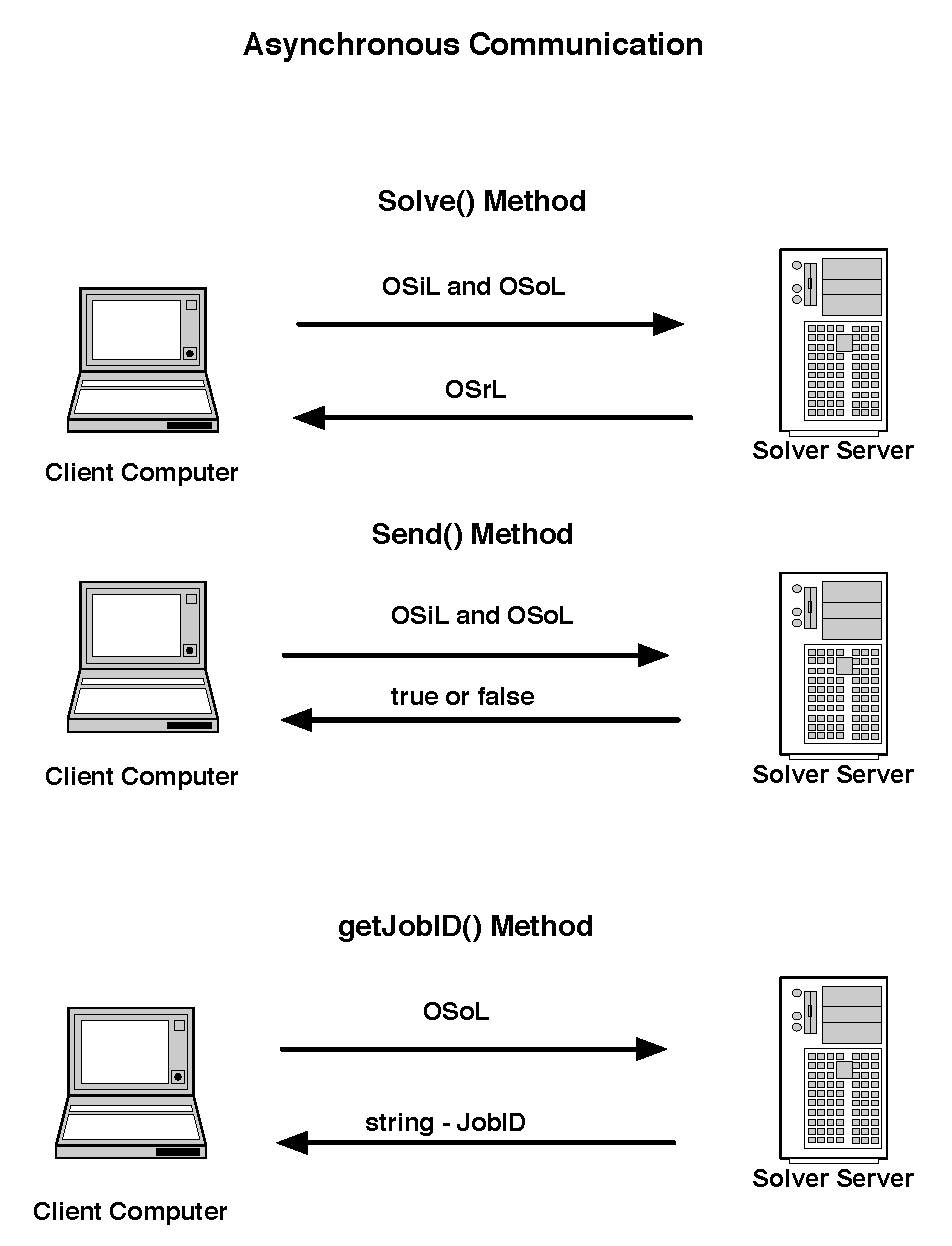
\includegraphics[scale=0.5]{\figurepath/asynchronous1.pdf}
\caption{Input and output for {\tt solve}, {\tt send}, and {\tt getJobID} methods.} 
\label{figure:async1}
\end{figure}


\begin{figure}[ht]
\centering
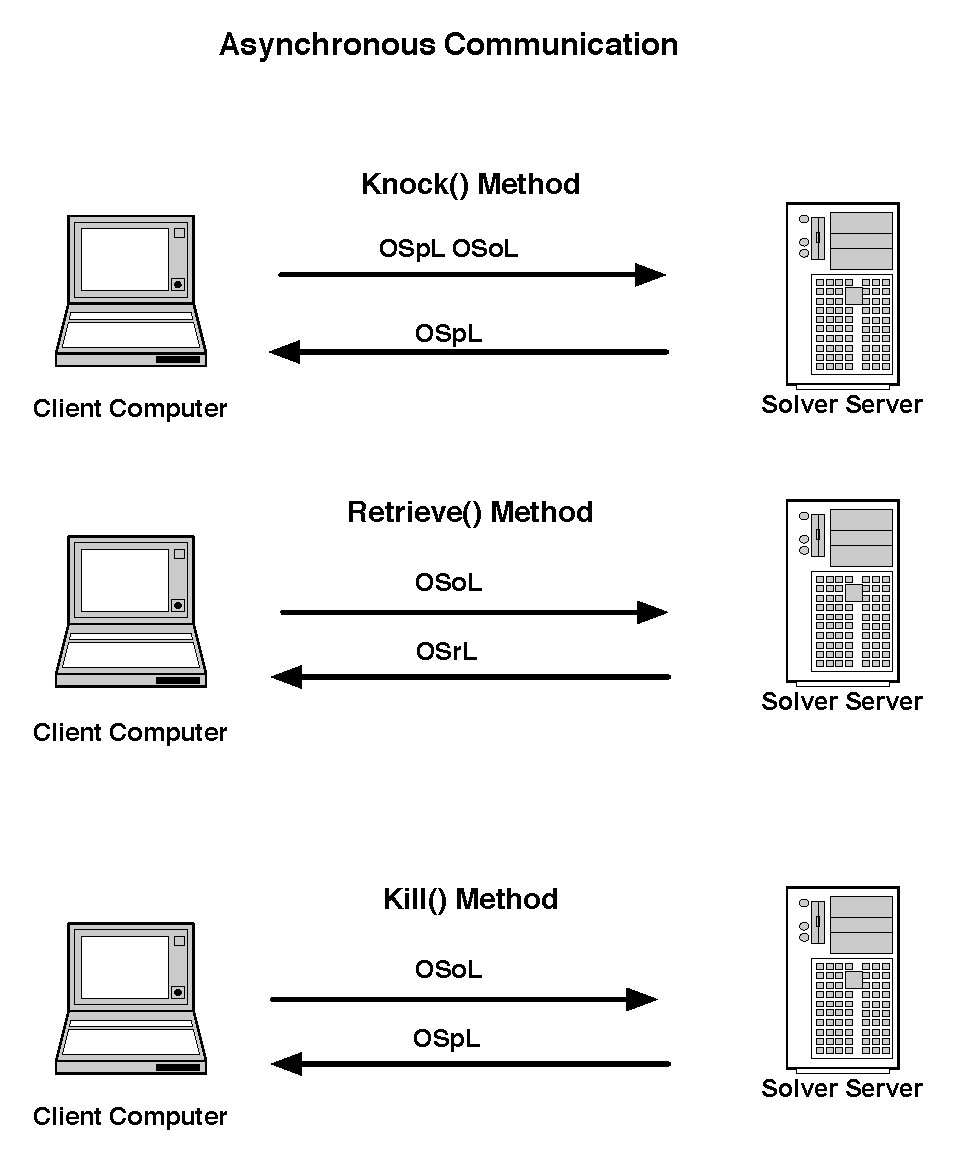
\includegraphics[scale=0.5]{\figurepath/asynchronous2.pdf}
\caption{Input and output for {\tt knock}, {\tt retrieve}, and {\tt kill} methods.} 
\label{figure:async2}
\end{figure}

\section{Setting up a Solver Service with Tomcat}\label{section:tomcat}





\section{Examples}

\subsection{AMPL Client:  Hooking AMPL to Solvers}

The {\tt amplClient} executable is designed to work with the AMPL program. See \url{www.ampl.com}. The {\tt amplClient} acts like an AMPL ``solver.'' The {\tt amplClient} is linked with the OS library and can be used to solve problems either remotely. In both cases the {\tt amplClient} uses the {\tt OSnl2osil} class to convert the AMPL generated nl file (which represents the problem instance) into the corresponding instance representation in the OSiL format.  

For example, assume that there is a problem instance, {\tt hs71.mod} in AMPL model format. To solve this problem locally by calling the {\tt amplClient} from AMPL first start AMPL and then execute the following commands. In this case we are assuming that the local solver used is {\tt Ipopt.} 

\begin{verbatim}
# take in problem 71 in Hock and Schittkowski 
# assume the problem is in the AMPL directory
model hs71.mod;
# tell AMPL that the solve is amplClient
option solver amplClient;
# now tell amplClient to use Ipopt
option amplClient_options "solver ipopt";
# the name of the nl file (this is optional)
write gtestfile;
# now solve the problem
solve;
\end{verbatim}

This will invoke {\tt Ipopt} locally and the result in OSrL format will be displayed on the screen. In order to call a remote solver service, after the command
\begin{verbatim}
option amplClient_options "solver ipopt";
\end{verbatim}
provide an option which has the address of the remote solver service.
\begin{verbatim}
option ipopt_options "http://128.135.130.17:8080/ipopt/IPOPTSolverService.jws";
\end{verbatim}

\subsection{CppAD:  Using the CppAD Algorithmic Differentiation Package}

\subsection{File Upload:  Using a File Upload Package}

\subsection{Instance Generator: Using the OSInstance API to Generate Instances}\label{subsection:exampleOSInstance}

\end{document}

